\chapter{Artificial Racing Agent}

In this chapter we will first analyze how racing drivers approach the task of car racing. We will then use this information to design a behavior of an autonomous agent and divide the problem into the subproblems of vehicle modeling, analysis of racing circuit topology, trajectory planning, and trajectory following. These subproblems will be described in more detail in the following chapters.

% todo: is this paragraph too broad? too much information about the other chapters?

\section{Racing Line}

When a human driver drives on a racing circuit, his or her task is to complete several laps around the circuit in a time period as short as possible. In order to minimize the lap times, the driver trades off the total distance the car travels for the average speed at which it moves. The trajectory of the vehicle through the racing track is sometimes referred to as the racing line and it depends on the shape of the track and on the vehicle. The driver will follow different racing lines for different vehicles on the same circuit based on many their different properties such as maximum speeds, acceleration, braking power, or the grip of the tires.

For a turn with a steady curvature there is a maximum speed at which a specific car can go and stay on the track. Exceeding this speed will cause a loss of friction between the tires and the road surface and the tires will not be able to exert enough lateral force to keep the car on the curve and the car will start to travel along a curve with a greater radius than the one commanded by the driver. This situation is called understeer or oversteer, depending on whether it was the front or rear wheels which lost the friction and which wheels are powered by the engine.

% todo: image of oversteer and understeer

On the other hand, for a constant vehicle speed, the vehicle can safely travel along any curve with a radius greater than the minimum safe radius. The driver will therefore try to follow curves with higher radii when going through corners but only to the point where the maximum safe speed reaches the maximum speed of the vehicle. Increasing the curvature when it is not possible to increase the speed adds to the distance the car travels but it does not increase the average speed and therefore leads to a higher lap time.

The trajectory of the vehicle as it goes through a corner can be split into several stages. First, the vehicle aligns itself to the outer edge of the track. Second, the vehicle must adjust its speed so it can safely stay on the curve. It is common to use the brakes mostly while the vehicle is moving straight to avoid locking the wheels in mid-turn. Third, the car starts turning at a turn-in point to go through the apex of the curve at the desired moment. Fourth, the vehicle goes through an apex, which is the point, where it is the closest to the inner edge of the track. Next, the vehicle starts exiting the corner and enters another part of the track.

There are two common ways of going through a corner, a classical one and one called late apex. The classical way of leaving the corner is to keep the constant curvature of the turn and to align the vehicle with the outer edge of the track. The late apex is achieved by starting to turn into the corner later and exiting the corner much closer to the inner edge of the track than the classical way. During the late apex turn, the vehicle slows down more before entering the corner and it straightens the line before hitting the apex allowing for greater exit speed. The comparison between these two lines can be seen in **todo figure**.

% figures to use: https://drivingfast.net/racing-line/#chapter-1

Another factor which affects the speed at which the driver can go through a corner is the shape of the track around the corner. When there is a straight stretch following the corner, the driver can maximize the speed at which the vehicle leaves the corner to increase the average speed. If there is another corner immediately after the first one, the driver must plan ahead and adjust the speed before entering the first corner to a level at which the exit speed of the first corner will be appropriate to go through the following corner.

From the description of the racing behavior of human expert drivers, it is apparent that the key components of choosing the optimal racing line are the knowledge of the behavior of the vehicle and the shape of the track. The knowledge of the track gives the driver an opportunity to plan how he or she is going to approach driving on the track. The driver can plan how to approach each individual corner and what speeds and turning radii are optimal and still safe.

\section{Artificial Agent}

\begin{defn}\label{def:rational_agent}
    A rational agent is an entity which gathers information from the environment through sensors and changes the state of the environment in order to maximize some performance measure.
\end{defn}

A racing driver can be thought of as a rational agent as defined in definition~\ref{def:rational_agent}. The driver observes the position of the vehicle on the racing track and the state of the vehicle as it moves along the track. He also observes the distance to the boundaries of the track and to any obstacles which can be present on the track. The driver reacts to these perceptions by giving control inputs to the vehicle through the steering wheel, brake and accelerator pedals, and shifting into different gears. The performance measure is the lack of collisions with the boundaries of the track or any obstacles on the track and minimizing of the lap time.

An artificial racing agent would use electronic sensors such a LIDAR, wheel encoders, an IMU, or a camera to observe the state of the environment. Based on this observation, the agent can estimate its state in the world and the state of other entities in the world, such as obstacles or opponents. Based on this information, the agent has to select a control input for the actuators of the vehicle.

The agent can use the information about its initial state and calculate a time-optimal racing line from this initial state through the whole circuit up to the finish line using a trajectory planning algorithm. Depending on the size of the circuit, this could be a computationally expensive operation. If later on there is a need to re-plan the trajectory during the race, because the vehicle could not follow the trajectory accurately and it is necessary to come up with a contingency plan, the vehicle might have to repeat the expensive calculation. Instead, the agent can analyze the shape of the circuit and identify the corners and focus its effort only on the next two or three corners ahead of him.

\subsection{Decision Process}

We will divide the decision process of the agent into several sub-problems: localization, track analysis and waypoint selection, trajectory planning, and trajectory following. The outputs of some of these sub-problems are inputs of the other and they form the nodes of a dependency graph of the decision process which is visualized in Figure~\ref{fig:racing_agent_diagram}. Vehicle modeling is also a separate problem and it is key to planning of feasible trajectories and for reliable trajectory following.

\begin{figure}[p]\centering
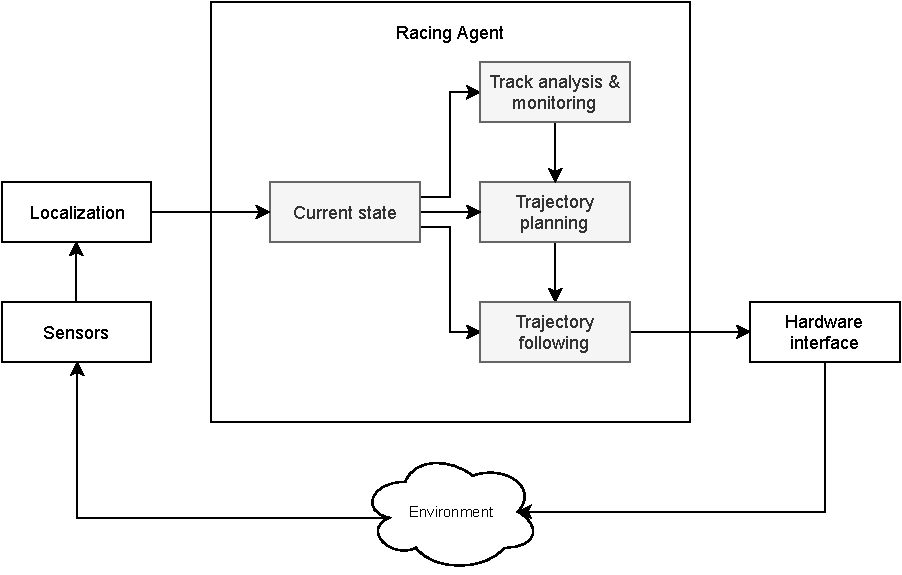
\includegraphics[width=125mm]{../img/racing_agent_diagram.pdf}
\caption{A diagram of the decision process of the racing agent.}
\label{fig:racing_agent_diagram}
\end{figure}

As the vehicle moves on the track, the agent needs to know its current position, orientation, and speed. A localization algorithm collects the data from different sensors and estimates the current state of the vehicle. The accuracy and the frequency of state updates depend greatly on the capabilities of the sensors and the processing power of the on-board computer. The responsibility of the localization algorithm is to publishes the vehicle state updates as frequently as possible and without a long delay between the time at which the data came from the sensors and at which it will be used as an input for trajectory planning and trajectory following.

Before the race begins, the agent analyses the track and finds all the corners and bends on the track and marks a coordinate of a point near the apex of the corner. Later during the race, it will keep track of which of these points was the last one which was reached and it selects the following $n$ waypoints as the next goal for trajectory planning. The constant $n\in\mathbb{N}$ is the planning lookahead of the agent.

The trajectory planning algorithm searches for a feasible trajectory from the last state of the vehicle estimated by the localization node through the waypoints selected by the track analysis. We expect the planning algorithm to find solutions quickly, because we reduced the size of the configuration space which is explored by the planning algorithm by limiting the lookahead distance to only a few corners ahead of the agent. The trajectory planning node will start planning a new trajectory as soon as it finishes planning the previous one as the initial conditions change as the vehicle follows the previous trajectory.

The latest reference trajectory and the current estimate of the state of the vehicle is used to calculate the next command for the actuators of the vehicle. In the ideal case, this trajectory following node will send the commands to the hardware at the maximum possible rate which the hardware is capable of. In practice we are limited by the rate at which we receive the state estimates from the localization node. The trajectory following node is also responsible for collision avoidance either by actively guiding the vehicle around the obstacles it might hit, or by slowing down the vehicle while waiting for a new reference trajectory.

\subsection{Track Analysis}

The definition of a racing circuit is given by an occupancy grid, initial coordinates of the vehicle in the grid and its heading direction, and at least two more checkpoints which define the direction in which the agent must drive along the circuit. An occupancy grid is a two dimensional table where the cells correspond to a square areas with an equal side length. The cells contain the information of whether it is safe to go through the area or if there is an obstacle in the area and the cell is not safe to go through.

The goal of the track analysis algorithm is to find interesting points of the track which split the track into smaller segments corresponding to stretches between the corners of the track. It would be hard to define how a corner and its apex look like in an occupancy grid, but we can make a simple observation and derive a simple algorithm which will produce good approximate solutions. We can inflate imaginary rubber walls with the thickness of a given safety radius of the vehicle along the edges of the track and loosely lay an imaginary string through the whole circuit. We can then start tightening the string and eventually it will take a form of alternating straight segments and parts, where it touches the rubber wall at an inner edge of a corner of a track. We can then remove the imaginary rubber walls and start walking along the string starting at the initial position of the vehicle. We will mark the furthest point which is directly visible from the place where we're standing. We will then imaginary walk to this point and repeat the process, until we can see the first point we marked. By directly visible we mean that it is possible to draw a line between the two points in the occupancy grid and it will not intersect a cell containing an obstacle between the two points. This thought process is visualized in figure~\ref{fig:thought_process} on different track layouts.

% figure with the analysis of the track

We will implement this process with a two step algorithm which will identify the apexes of corners and points along long winding bends. The first step will be to find the shortest path through the grid which starts at the initial position of the vehicle, and which goes through the checkpoints in the correct order and at any point it does not come closer to an obstacle than to a distance of the safety radius. The second step will simply traverse the path once and select a subsequence of the points such that for two consecutive points $A$ and $B$, $B$ was the last point of the points immediately following $A$ on the original track which are directly visible from $A$.

The shortest path search can be various ways. The simplest approach would be to use a simple grid search on the occupancy grid. An interesting alternative is the Space Exploration algorithm described by Chao Chen \cite{SEHS} which explores the grid using circles of variable radii which depend on the distance to the closest obstacle. The outline of the algorithm is described in algorithm~\ref{alg:space_exploration}.

\begin{algorithm}[]
\SetAlgoLined
\KwResult{Shortest path through the occupancy grid}
 $r_i\set MaxRadius(i)$\;
 $O\gets\{(i, r_i)\}$\;
 $C\gets\emptyset$\;
 \While{$O \neq \emptyset$}{
  $(c, r)\gets Top(O)$\;
  $O\getsO-\{(c, r)\}$\;
  
  \eIf{condition}{
   instructions1\;
   instructions2\;
   }{
   instructions3\;
  }

  $C\getsC\cup\{(c, r)\}$\;
 }
 \caption{Space Exploration}
 \label{alg:space_exploration}
\end{algorithm}

Algorithm.png 

% SELECTION OF VISIBLE POINTS

% do I need to prove 

